%!TEX root = ../../controlbook.tex

\begin{figure}[htb]
  % Requires \usepackage{graphicx}
  \centering
  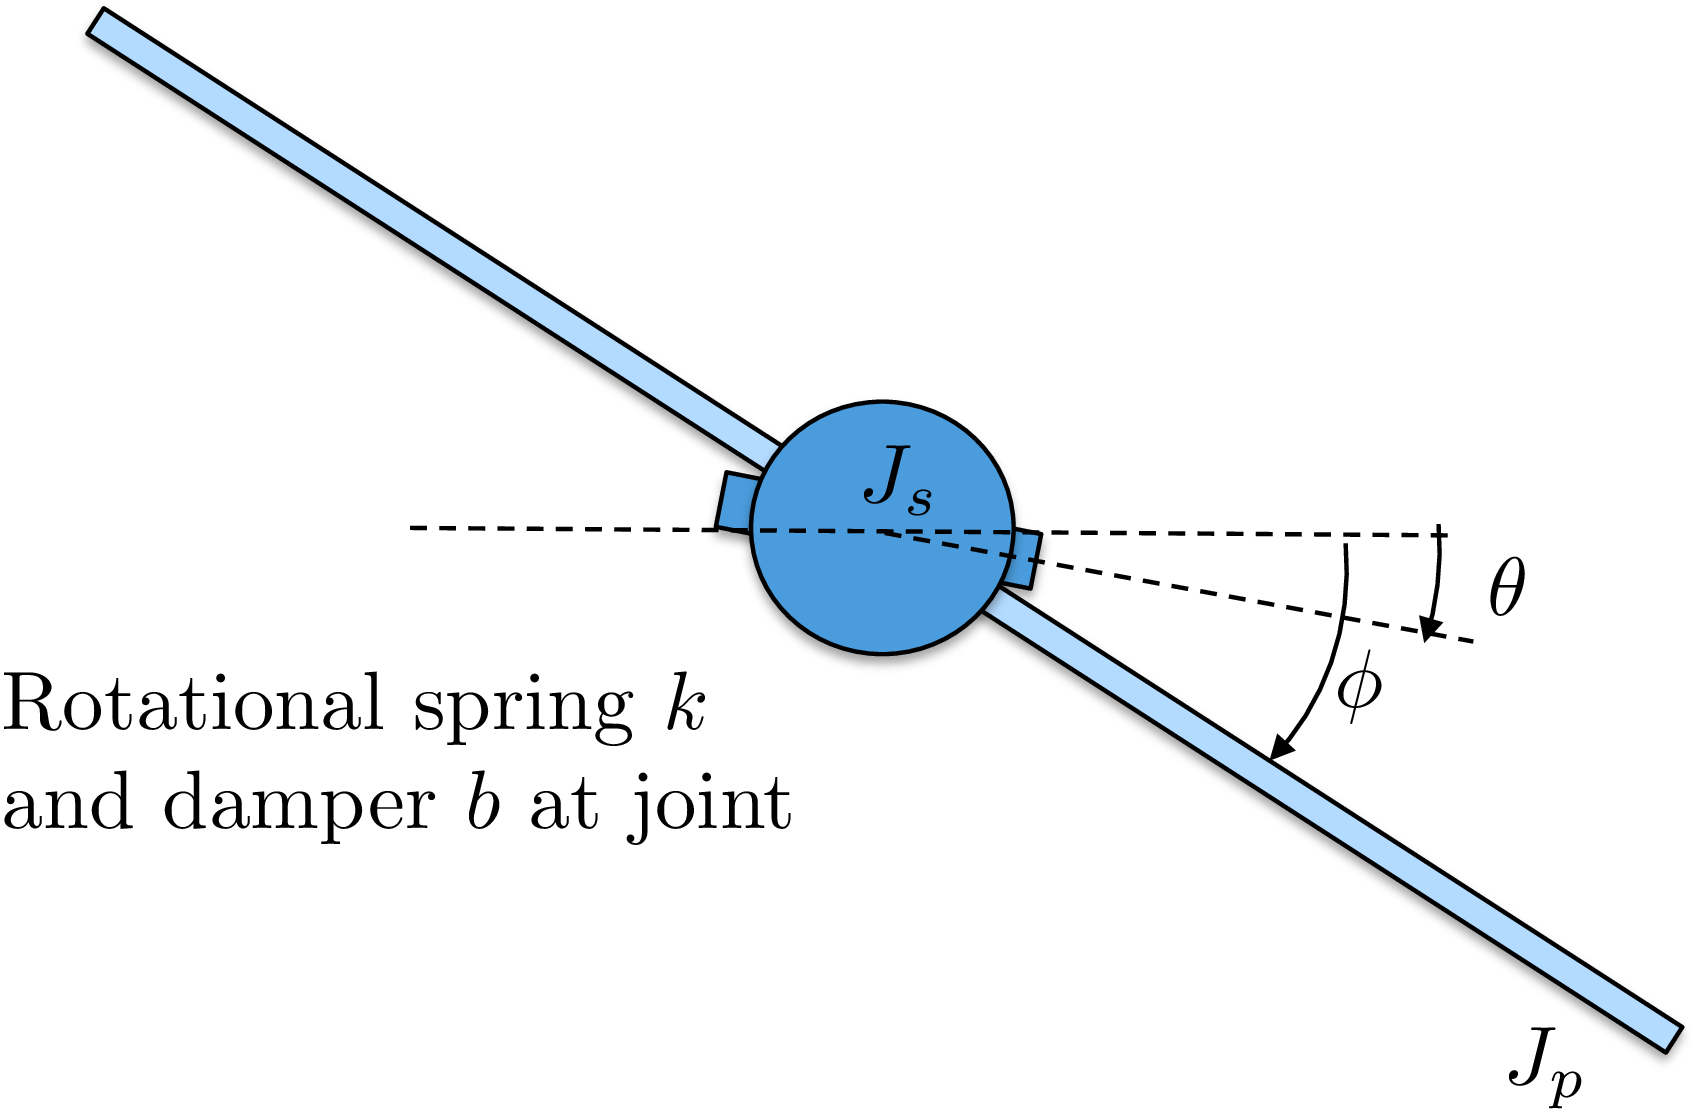
\includegraphics[width=0.5\textwidth]{6_design_studies/figures/hw_satellite_defn.pdf}
  \caption{Satellite with flexible solar panels.}
  \label{fig:int_satellite_defn}
\end{figure}

%\begin{figure}[tb!]
%\figureboxscale{0.5}{6_design_studies/figures/hw_satellite_defn}
%{Satellite with flexible solar panels.\label{fig:int_satellite_defn}}
%\end{figure}

Figure~\ref{fig:int_satellite_defn} shows a simplified version of a satellite with flexible solar panels.  We will model the flexible panels using a rigid sheet with moment of inertia $J_p$ connected to the main satellite body by a torsional compliant element with spring constant $k$ and damping constant $b$.  The moment of inertia of the satellite is $J_s$.  The angle of the satellite body from the inertial reference is $\theta$ and the angle of the panel from the inertial reference is denoted as $\phi$.  Thrusters are used to command an external torque of $\tau$ about the axis of the satellite body.

The physical constants are $J_s=5$~kg~m$^2$, $J_p=1$~kg~m$^2$, $k=0.15$~N~m, $b=0.05$~Nms.  The torque is limited by $\abs{\tau}\leq 5$~Nm.